
\section{Prueba 2}


\subsection{Red de inferencia}
\begin{center}
	\tikzstyle{regla}= [rectangle,draw,black,fill=blue!15]
	\tikzstyle{hecho}= [rectangle,draw,black,fill=black!15]
	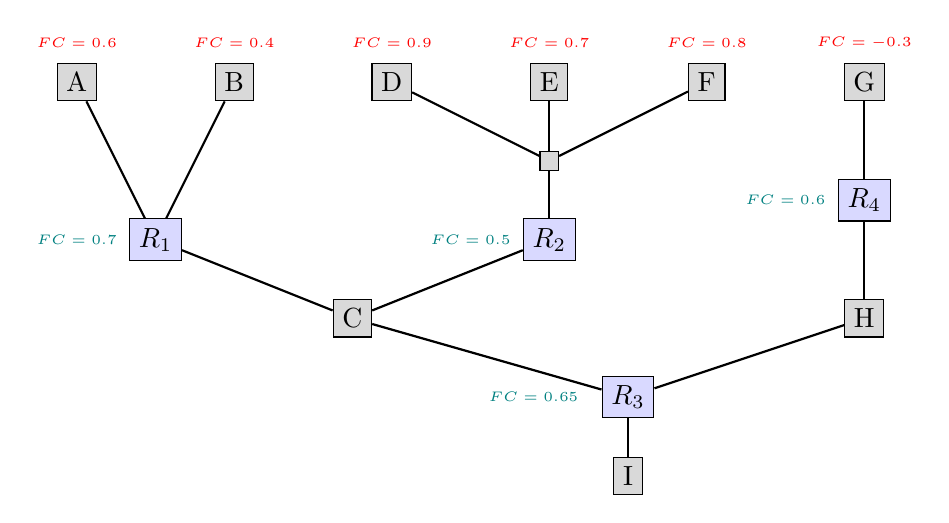
\begin{tikzpicture}
		
		\node (a) at (0,5) [hecho] {A};
		\node at (0,5.5) {\color{red}{\tiny{$FC=0.6$}}};

		\node (b) at (2,5) [hecho] {B};
		\node at (2,5.5) {\color{red}{\tiny{$FC=0.4$}}};

		\node (c) at (3.5,2) [hecho] {C};

		\node (d) at (4,5)[hecho] {D};
		\node at (4,5.5) {\color{red}{\tiny{$FC=0.9$}}};

		\node (e) at (6,5)[hecho] {E};
		\node at (6,5.5) {\color{red}{\tiny{$FC=0.7$}}};

		\node (f) at (8,5)[hecho] {F};
		\node at (8,5.5) {\color{red}{\tiny{$FC=0.8$}}};

		\node (g) at (10,5)[hecho] {G};
		\node at (10,5.5) {\color{red}{\tiny{$FC= -0.3$}}};

		\node (h) at (10,2)[hecho] {H};

		\node (i) at (7,0)[hecho] {I};

		\node (d/e/f) at (6,4)[hecho] {};

		\node (r1) at (1,3) [regla] {$R_{1}$};
		\node at (0,3) {\color{teal}{\tiny{$FC=0.7$}}};
		\node (r2) at (6,3) [regla] {$R_{2}$};
		\node at (5,3) {\color{teal}{\tiny{$FC=0.5$}}};
		\node (r3) at (7,1) [regla] {$R_{3}$};
		\node at (5.8,1) {\color{teal}{\tiny{$FC=0.65$}}};
		\node (r4) at (10,3.5) [regla] {$R_{4}$};
		\node at (9,3.5) {\color{teal}{\tiny{$FC=0.6$}}};

		\path[black,thick] (a) edge[] node {} (r1);
		\path[black,thick] (b) edge[] node {} (r1);
		\path[black,thick] (r1) edge[] node {} (c);
	
		\path[black,thick] (d) edge[] node {} (d/e/f);
		\path[black,thick] (e) edge[] node {} (d/e/f);
		\path[black,thick] (f) edge[] node {} (d/e/f);
		\path[black,thick] (d/e/f) edge[] node {} (r2);
		\path[black,thick] (r2) edge[] node {} (c);

		\path[black,thick] (g) edge[] node {} (r4);
		\path[black,thick] (r4) edge[] node {} (h);

		\path[black,thick] (c) edge[] node {} (r3);
		\path[black,thick] (h) edge[] node {} (r3);
		\path[black,thick] (r3) edge[] node {} (i);

	\end{tikzpicture}
\end{center}
\par Esta red de inferencia se debe interpretar de arriba a abajo.
Los rectángulos azules son las reglas, los grises que están ligados por encima 
de ellas son sus antecedentes, si estos antecedentes convergen en un cuadrado 
quiere decir que es la conjunción de esos literales, en caso contrario son disyunciones
o simplemente un literal. Los rectángulos grises que cuelgan de las reglas 
son sus consecuentes respectivamente. Además, incluyo los factores de certeza propocionados por
la Base de hechos y la Base de Conocimiento iniciales.

\subsection{Proceso de inferencia}
\begin{listing}[language=Pascal]
(Razonamiento dirigido por Metas)
Objetivo: I
Proceso de Inferencia: 
  ###########################
  # Llamada (1) a verificar #
  ###########################
	Verificar(I,{A,B,D,E,F,G}) // Recursion 
	Conjunto Conflicto={R3} // I es consecuente de estas reglas
	R={R3} // Seleccionar regla R3
	Eliminar R3 ---> Conjunto Conflicto={}
	NuevasMetas={C,H} // Antecedentes de R3; Verificado = true
	Meta=C // Seleccionar C de NuevasMetas
	NuevasMetas={H} // Eliminar C de NuevasMetas

  ###########################
  # Llamada (2) a verificar #
  ###########################
	Verificar(C,{A,B,D,E,F,G}) // Recursion 
	Conjunto Conflicto={R1,R2} // C es consecuente de estas reglas
	R={R1} // Seleccionar regla R1
	Eliminar R1 ---> Conjunto Conflicto={R2}
	NuevasMetas={A,B} // Antecedentes de R1; Verificado = true
	Meta=A // Seleccionar A de NuevasMetas
	NuevasMetas={B} // Eliminar A de NuevasMetas
  ###########################
  # Llamada (3) a verificar #
  ###########################
	Verificar(A,{A,B,D,E,F,G}) ---> true // Recursion: A en BH
	BH={A,B,D,E,F,G}
	Meta=B // Seleccionar B de NuevasMetas
	NuevasMetas={} // Eliminar B de NuevasMetas
  ###########################
  # Llamada (4) a verificar #
  ###########################
	Verificar(B,{A,B,D,E,F,G}) ---> true // Recursion: B en BH
	BH={A,B,D,E,F,G}
	(CASO 1): Combinacion de antecedentes de R1
	 FC(A o B)=min(FC(A),FC(B))=0.6
	(CASO 3): Combinacion de la evidencia con la regla R1
	 FC(C{R1})=0.7*max(0,FC(A o B))=0.42
	Conjunto Conflicto={R2} // C es consecuente de estas reglas
	R={R2} // Seleccionar regla R2
	Eliminar R2 ---> Conjunto Conflicto={}
	NuevasMetas={D,E,F} // Antecedentes de R2; Verificado = true
	Meta=D // Seleccionar D de NuevasMetas
	NuevasMetas={E,F} // Eliminar D de NuevasMetas
  ###########################
  # Llamada (5) a verificar #
  ###########################
	Verificar(D,{A,B,D,E,F,G}) ---> true // Recursion: D en BH
	BH={A,B,D,E,F,G}
	Meta=E // Seleccionar E de NuevasMetas
	NuevasMetas={F} // Eliminar E de NuevasMetas
  ###########################
  # Llamada (6) a verificar #
  ###########################
	Verificar(E,{A,B,D,E,F,G}) ---> true // Recursion: E en BH
	BH={A,B,D,E,F,G}
	Meta=F // Seleccionar F de NuevasMetas
	NuevasMetas={} // Eliminar F de NuevasMetas
  ###########################
  # Llamada (7) a verificar #
  ###########################
	Verificar(F,{A,B,D,E,F,G}) ---> true // Recursion: F en BH
	BH={A,B,D,E,F,G}
	(CASO 1): Combinacion de antecedentes de R2
	 FC(D y E y F)=min(FC(D),FC(E),FC(F),)=0.7
	(CASO 3): Combinacion de la evidencia con la regla R2
	 FC(C{R2})=0.5*max(0,FC(D y E y F))=0.35
	(CASO 2): Combinacion de las reglas R1 y R2
	 FC(C)=FC(C{R1}) + FC(C{R2})*(1-FC(C{R1}))=0.623
	BH={A,B,C,D,E,F,G} // Insertar C a la Base de Hechos
	Meta=H // Seleccionar H de NuevasMetas
	NuevasMetas={} // Eliminar H de NuevasMetas
  ###########################
  # Llamada (8) a verificar #
  ###########################
	Verificar(H,{A,B,C,D,E,F,G}) // Recursion 
	Conjunto Conflicto={R4} // H es consecuente de estas reglas
	R={R4} // Seleccionar regla R4
	Eliminar R4 ---> Conjunto Conflicto={}
	NuevasMetas={G} // Antecedentes de R4; Verificado = true
	Meta=G // Seleccionar G de NuevasMetas
	NuevasMetas={} // Eliminar G de NuevasMetas
  ###########################
  # Llamada (9) a verificar #
  ###########################
	Verificar(G,{A,B,C,D,E,F,G}) ---> true // Recursion: G en BH
	BH={A,B,C,D,E,F,G}
	(CASO 3): Combinacion de la evidencia con la regla R4
	 FC(H{R4})=0.6*max(0,FC(G))=0
	BH={A,B,C,D,E,F,G,H} // Insertar H a la Base de Hechos
	(CASO 1): Combinacion de antecedentes de R3
	 FC(C o H)=min(FC(C),FC(H))=0.623
	(CASO 3): Combinacion de la evidencia con la regla R3
	 FC(I{R3})=0.65*max(0,FC(C o H))=0.40495
	BH={A,B,C,D,E,F,G,H,I} // Insertar I a la Base de Hechos
Return TRUE	
\end{listing}

\subsection{Objetivo obtenido por SBR-FC}
\begin{center}
\par -------------------- Hecho (I) ---------------------
\par Hecho (nomHecho): I
\par Hecho (facCerBH): 0.40495
\par --------------------------------------------------------
\end{center}

\subsection{Cuestión}
\begin{ejer}
	\textbf{Prueba 2.} En un momento determinado se tiene la siguiente información sobre los hechos:\\
	Se está cumpliendo \texttt{A} con grado 0.6, \texttt{B} con grado 0.4, \texttt{D} con grado 0.9, 
	\texttt{E} con grado 0.7, \texttt{F} con grado 0.8 y \texttt{G} no se está cumpliendo con grado 0.3. \\
	Con esta información, ¿con qué grado se cumple \texttt{I}?
\end{ejer}
\par Solución: Se cumple con grado 0.40495.